% !TEX TS-program = pdflatex
% !TEX encoding = UTF-8 Unicode

% This is a simple template for a LaTeX document using the "article" class.
% See "book", "report", "letter" for other types of document.

\documentclass[11pt]{article} % use larger type; default would be 10pt

%\usepackage[utf8]{inputenc} % set input encoding (not needed with XeLaTeX)
\usepackage[utf8]{inputenc}
\usepackage{polski}
\usepackage[polish]{babel}

%%% Examples of Article customizations
% These packages are optional, depending whether you want the features they provide.
% See the LaTeX Companion or other references for full information.

%%% PAGE DIMENSIONS
\usepackage{geometry} % to change the page dimensions
\geometry{a4paper} % or letterpaper (US) or a5paper or....
% \geometry{margin=2in} % for example, change the margins to 2 inches all round
% \geometry{landscape} % set up the page for landscape
%   read geometry.pdf for detailed page layout information

\usepackage{graphicx} % support the \includegraphics command and options

% \usepackage[parfill]{parskip} % Activate to begin paragraphs with an empty line rather than an indent

%%% PACKAGES
\usepackage{booktabs} % for much better looking tables
\usepackage{array} % for better arrays (eg matrices) in maths
\usepackage{paralist} % very flexible & customisable lists (eg. enumerate/itemize, etc.)
\usepackage{verbatim} % adds environment for commenting out blocks of text & for better verbatim
\usepackage{subfig} % make it possible to include more than one captioned figure/table in a single float
\usepackage{hyperref}
\usepackage{makeidx}
\usepackage{graphicx}
\usepackage{amsmath}
\usepackage{amsthm}
\usepackage{amsfonts}
% These packages are all incorporated in the memoir class to one degree or another...

%%% HEADERS & FOOTERS
\usepackage{fancyhdr} % This should be set AFTER setting up the page geometry
\pagestyle{fancy} % options: empty , plain , fancy
\renewcommand{\headrulewidth}{0pt} % customise the layout...
\lhead{}\chead{}\rhead{}
\lfoot{}\cfoot{\thepage}\rfoot{}

% Theorem Styles
\newtheorem{theorem}{Twierdzenie}[section]
\newtheorem{lemma}[theorem]{Lemat}
\newtheorem{proposition}[theorem]{Założenie}
\newtheorem{corollary}[theorem]{Wniosek}
% Definition Styles
\theoremstyle{definition}
\newtheorem{definition}{Definicja}[section]
\newtheorem{example}{Przykład}[section]
\theoremstyle{remark}
\newtheorem{remark}{Uwaga}

%%% SECTION TITLE APPEARANCE
\usepackage{sectsty}
\allsectionsfont{\sffamily\mdseries\upshape} % (See the fntguide.pdf for font help)
% (This matches ConTeXt defaults)

%%% ToC (table of contents) APPEARANCE
\usepackage[nottoc,notlof,notlot]{tocbibind} % Put the bibliography in the ToC
\usepackage[titles,subfigure]{tocloft} % Alter the style of the Table of Contents
\renewcommand{\cftsecfont}{\rmfamily\mdseries\upshape}
\renewcommand{\cftsecpagefont}{\rmfamily\mdseries\upshape} % No bold!

%%% END Article customizations

%%% The "real" document content comes below...

\title{Wprowadzenie do \LaTeX}
\author{Marcin Dembowski}
\date{\today} % Activate to display a given date or no date (if empty),
         % otherwise the current date is printed 

\begin{document}
\maketitle
\begin{abstract}
Ten krótki dokument pozwala wyjaśnić podstawy korzystania z systemu \LaTeX. Przedstawia sposób instlacji oraz tworzenia dokumentów wykorzystujących pakiety matematyczne. Każdy krok zawiera listę odnośników, które szczegółowiej wyjaśniają dane zagadnienie.
\end{abstract}

\section{Czym jest \LaTeX}
\LaTeX - jest oprogramowaniem służącym do automatyzacji składu tekstu oraz związany z nim język znaczników służący do formatowania dokumentów tekstowych i tekstowo-graficznych \cite{wikipedia_latex}. Poprawnie \LaTeX\ powinno wymawiać się jako \textit{lejtech}, nigdy latex lub lejtek. 
Czemu nie jest wykorzystywany pakiet Office? Otóż, nie każdy go posiada, nie wszędzie dokument wygląda tak samo - szczególnie ten, który został utworzony w innym pakiecie. Największą zaletą \LaTeX\ jest \textit{prostota} pisania skomplikowanych wzorów matematycznych i osadzania grafik i odnośników. Jedna uwaga, na początku sposób tworzenia tego typu dokumentów może być uciążliwy jednak z biegiem czasu uciążliwsze staje się używanie myszki.
\section{Co wybrać}

Dostępnych jest wiele dystrybucji, projektów i edytorów wspierających pisanie dokumentów.

\begin{description}
	\item[LaTeX]
		\href{http://www.latex-project.org/}{Strona główna projektu}.
  \item[MikTeX]
  		\href{http://www.miktex.org/}{Dystrybucja dla systemu Windows.}
  \item[LEd]
  		\href{http://www.latexeditor.org/}{Edytor dla systemów Windows.}
  \item[TeXstudio]
  		\href{http://texstudio.sourceforge.net/}{Edytor dla systemów Windows i innych.}
  \item[TeXworks]
  		\href{http://www.tug.org/texworks/}{Edytor dla systemów Windows.}\ldots
\end{description}

\subsection{TeXworks - nasza dystrybucja}
Wszystkie instrukcje i przykłady będą bazowały na dystrybucji \textit{MikTeX} oraz po części edytorze \textit{TeXworks}, który jest instalowany wraz z powyższą dystrybucją. Zalecane jest jednak zainstalowanie \textit{TeXstudio}, o którym powiemy sobie dalej.

\subsubsection{Instalacja i konfiguracja}
Instalacja jest bardzo prosta i przyjemna. Wystarczy ściągnąć i zainstalować dystrybucję MikTeX ze strony \url{http://www.latex-project.org/} i postępować według instrukcji instalatora. Nawet dostępny jest \href{http://miktex.org/howto/install-miktex}{przewodnik na stronie}, który opisuje krok po kroku jak należy postępować z instalacją.
\begin{remark}
	Zalecam instalowanie aplikacji w języku angielskim. Dlaczego?
	\begin{itemize}
		\item Zaznajamiając się z interfejsem użytkownika w języku angielskim, uczysz się także tego języka
		\item Szybciej można znaleźć odwpowiedź na wiele pytań wpisując właśnie pytanie w języku angielskim
		\item Nawet jeżeli nie czujesz się na siłach w języku angielskim również zainstaluj aplikacje w języku angielskim - w domu masz sporo czasu aby poszukać tłumaczenie oraz uczyć się tego języka
	\end{itemize}
\end{remark}
\begin{figure}[!ht]
	\centering
	\makebox[\textwidth]{
		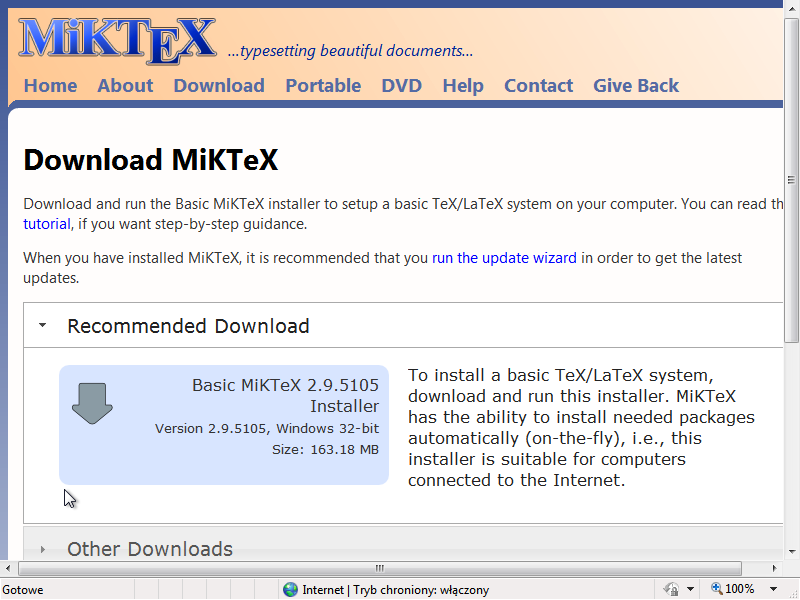
\includegraphics[width=.5\paperwidth]{MikTeX}
	}
	\caption{Strona główna projektu MikTex.}
\end{figure}
Instalator nie jest to jednak pełną dystrybucją, a jego wersją okrojoną - nie będzie nam to przeszkadzało. Wszystkie brakujące pakiety, które nie są dostępne wraz z instalatorem, zostaną dociągnięte podczas kompilacji gdy zajdzie taka potrzeba.

\subsubsection{Tworzenie dokumentów}
Wraz z instalacją MikTeX, instalowany jest również edytor TexWorks. Posiada on już kilka szablonów, które mogą zostać użyte jako podstawa tworzenia artykułu czy nawet prezentacji. Szablony te dostępne są z menu \textit{Plik} i pozycji \textit{Nowy na podstawie szablonu...}

Aktualnie czytany dokument, został utworzony właśnie na podstawie takiego szablonu i jest on dostępny na mojej stronie internetowej pod kategorią \href{http://marcindembowski.wordpress.com/category/studies/}{Studies}.

\subsubsection{TeXstudio}
Innym ciekawym edytorem jest \href{http://texstudio.sourceforge.net/}{TeXstudio}. Posiada on o wiele bardziej rozbudowany mechanizm wspomagający przeglądanie i pisanie dokumentu. Wyróżnia go podpowiadanie i kompletowanie składni oraz zasobnik posiadający listę symboli matematycznych.

\begin{remark}
	Edytor może mieć problemy z wprowadzaniem polskich znaków. W tym celu należy w menu \textit{Opcje} wybrać \textit{Konfiguruj TeXstudio}, a następnie w lewej części wybrać \textit{Skróty}. Należy usunąć skrót wybierając w drzewie menu \textit{Plik}, \textit{Zapisz jako...}, następnie dwa razy klikając w przecięciu z kolumną \textit{Aktualny skrót}.

	\begin{figure}[!ht]
		\centering
		\makebox[\textwidth]{
			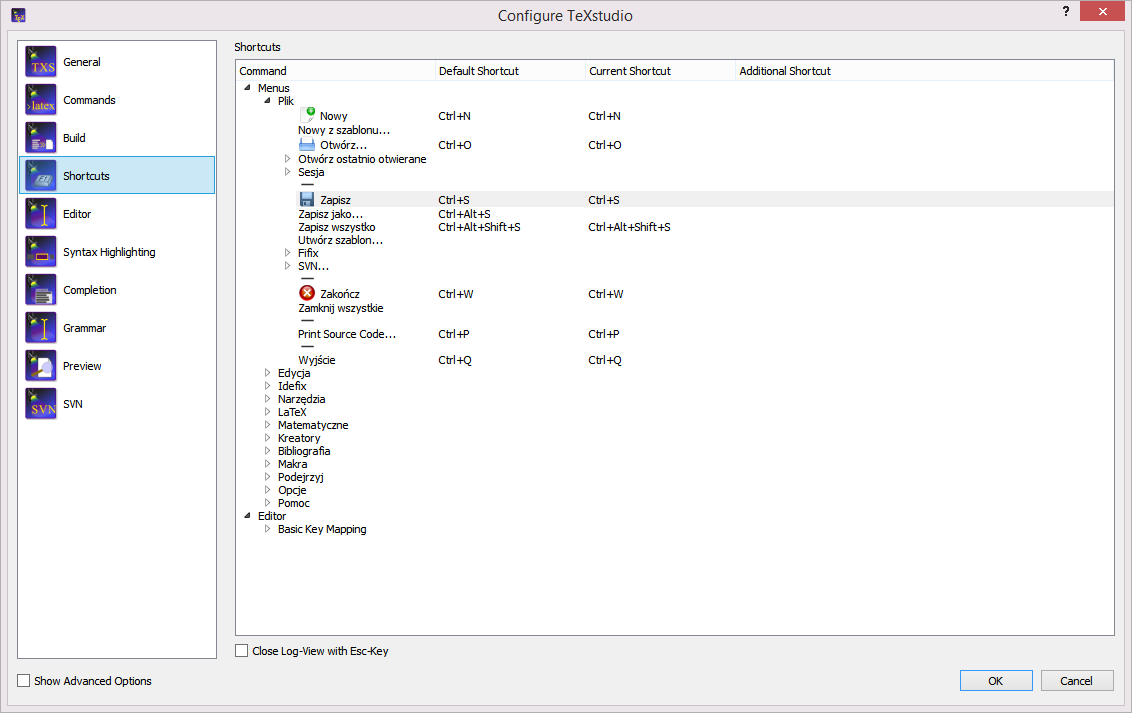
\includegraphics[width=.5\paperwidth]{TeXstudioSkroty}
		}
		\caption{Usuwanie skrótu zapisz jako powodującego blokadę litery 'ś'.}
	\end{figure}
\end{remark}

\section{Podstawy - matematyka}
Rozdział ten jedynie pokrótce pokaże niektóre możliwości \LaTeX w dziedzinie matematyki. Tworząc różnego rodzaju definicje, formuły, wzory czy wyjaśnienia, należy zachować szczególną dbałość o wygląd końcowy - czytanie równań, które są starannie wyjaśnione \ref{przyklad_rownania} oraz sformatowane jest o wiele przyjemniejsze, niż zastanawianie się nad położeniem początku i końca równania.

\begin{definition}[Opcjonalna nazwa definicji]
Treść definicji.
\begin{equation} \label{przyklad_rownania}
\begin{split}
LHS(x) & = max\{ A(x), min\{A(x), B(x) \} \} \\
 & = \begin{cases}
 			A(x) \le B(x)&: A(x) \\
 			B(x) \le A(x)&: A(x)
 		\end{cases} \\
 & = A(x)
\end{split}
\end{equation}
\end{definition}

\begin{theorem}
$\forall n\in \mathbb{N}$, prawdziwa jest nierówność:
\[
\sum^{n}_{i=0} \frac{1}{n+i} \ge \frac{2}{3}
\]
\end{theorem}
\begin{example}
\begin{equation}
\begin{split}
LHS(x) &= min\left(\frac{1}{2} + max\left(\frac{1}{2}+\frac{2}{3}-1,0\right)\right) \\
	&=\frac{5}{6}\ne \frac{1}{2}
\end{split}
\end{equation}
\end{example}
\subsection{Dalsza pomoc}
W sieci dostępnych jest sporo materiałów, które wyjaśniają sposób tworzenia i edytowania dokumentów. Pierwszą pomocą jest zawsze wyszukiwarka \href{http://google.pl}{Google} - najlepiej pytać ją w języku angielskim. Skupiając się jednak na części matematycznej, warte uwagi są pozycje \cite{sharelatex}, \cite{online_tutorial}, \cite{wikibooks_mathematics}.
%%
%% Wikipedia
%%
\begin{thebibliography}{1}

	\bibitem{wikipedia_latex} {\em \href{http://pl.wikipedia.org/wiki/LaTeX}{LaTeX}} Wikipedia.
	\bibitem{latex_wprowadzenie} {\em Nie za krótkie wprowadzenie do systemu \LaTeX}
	\bibitem{online_tutorial} { \href{http://www.tug.org.in/tutorials.html}{Online tutorials on \LaTeX}}
	\bibitem{wikibooks_mathematics}{ \href{http://en.wikibooks.org/wiki/LaTeX/Mathematics}{Wikibooks Mathematics}}
	\bibitem{sharelatex}{ \href{https://www.sharelatex.com/learn}{Share LaTeX}}
\end{thebibliography}
\end{document}
